\subsection{Prospective new-task execution and complete comparisons}\label{app:new-family-results}
This extension was declared before its outcomes: six settings, five methods and six candidates per method. Every formal run uses seed 42 and 1000 complete epochs. Configuration selection uses terminal-100 validation metrics. A comparison appears only after all 30 declared candidates have completed or recorded failure; failures have no fabricated endpoint. A method with no complete candidate has no selected score. Negative outcomes and every declared setting remain in this record.
\begin{table}[htbp]\centering\footnotesize\setlength{\tabcolsep}{3pt}\caption{Execution coverage of every declared new setting. Counts are configurations, not quality wins; failed candidates remain visible.}\begin{adjustbox}{max width=\linewidth}
\begin{tabular}{llrrrr}\toprule Family & Setting & Complete & Running & Pending & Failed\\\midrule
forecasting & ETTh1 / H24 & 30 & 0 & 0 & 0 \\
forecasting & ETTh2 / H24 & 30 & 0 & 0 & 0 \\
recommendation & MovieLens100K / ratings & 30 & 0 & 0 & 0 \\
recommendation & MovieLens1M / ratings & 30 & 0 & 0 & 0 \\
sensor\_drift & Gas sensors / fine-tuning & 30 & 0 & 0 & 0 \\
sensor\_drift & Gas sensors / replay & 30 & 0 & 0 & 0 \\
\bottomrule\end{tabular}
\end{adjustbox}\end{table}
\FloatBarrier
{\footnotesize\setlength{\tabcolsep}{3pt}\begin{longtable}{llrrrrr}\caption{All fully searched new settings. Each displayed method independently selects among six candidates on validation. Values are terminal-100 test metrics; MSE and RMSE are lower-is-better, accuracy is higher-is-better. No setting is omitted according to outcome.}\label{tab:new-families-complete}\\\toprule Setting & Metric & STRATA & Single-G & AdamW & GaLore & Indep.\\\midrule\endfirsthead\toprule Setting & Metric & STRATA & Single-G & AdamW & GaLore & Indep.\\\midrule\endhead
ETTh1 / H24 & MSE & \cellcolor{oursbg}0.89922 & 0.88655 & 0.86679 & \textbf{0.76942} & 0.90163 \\
ETTh2 / H24 & MSE & \cellcolor{oursbg}\textbf{1.74404} & 2.37970 & 2.16884 & 1.79170 & 2.18874 \\
MovieLens100K / ratings & RMSE & \cellcolor{oursbg}0.96949 & 1.00529 & \textbf{0.93295} & 0.95778 & 1.01755 \\
MovieLens1M / ratings & RMSE & \cellcolor{oursbg}1.05052 & 1.09444 & 0.98066 & \textbf{0.91712} & 1.08146 \\
Gas sensors / fine-tuning & acc & \cellcolor{oursbg}0.85453 & 0.85375 & 0.82335 & \textbf{0.90656} & 0.80659 \\
Gas sensors / replay & acc & \cellcolor{oursbg}0.96506 & 0.96409 & \textbf{0.96536} & 0.96232 & 0.96343 \\
\bottomrule\end{longtable}}
\clearpage
\paragraph{ETTh1 / H24 complete search.} Primary metric: MSE. Recorded candidate failures: STRATA 0, Single-G 0, AdamW 0, GaLore 0, Independent 0. Shared-CPU wall time is not isolated throughput; tensor-state size is distinct from peak memory.
\begin{table}[htbp]\centering\caption{\textbf{ETTh1 / H24: selected configurations and stored state.} Each method selects among six candidates on validation. Bold marks the best validation/test value; the green row identifies STRATA. Pareto status uses test quality and stored state, not peak memory.}\begin{adjustbox}{max width=\linewidth}
\begin{tabular}{lrrrrrl}\toprule Method & lr & $\xi$ & Val & Test & State MiB & Pareto\\\midrule
\rowcolor{oursbg}
STRATA & 3e-04 & 0.001 & 0.91637 & 0.89922 & 0.792 & \rwcross \\
Single-G & 3e-04 & 0.001 & 1.06275 & 0.88655 & 0.585 & \rwcross \\
AdamW & 1e-02 & -- & 0.94111 & 0.86679 & 2.146 & \rwcross \\
GaLore & 1e-04 & -- & \textbf{0.73812} & \textbf{0.76942} & 0.377 & \rwcheck \\
Independent & 3e-04 & 0.1 & 1.04792 & 0.90163 & 0.751 & \rwcross \\
\bottomrule\end{tabular}
\end{adjustbox}\end{table}
\begin{figure}[!htbp]\centering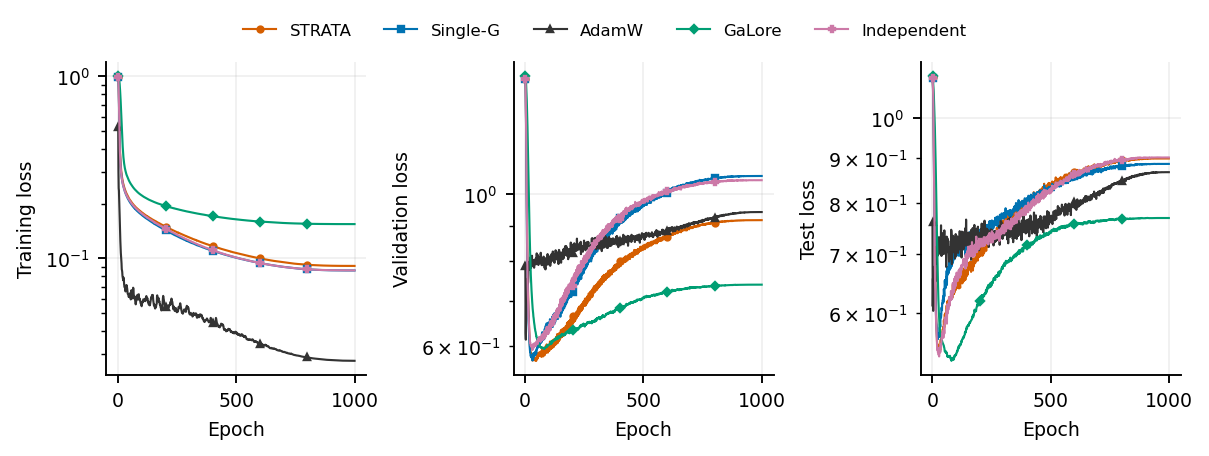
\includegraphics[width=.98\linewidth]{figures/fig_new_family_edb567be48.png}\caption{Complete ETTh1 / H24 loss trajectories. Left to right: training, validation, and test loss. Selection uses validation only after all candidates finish or record failure. All five methods and adverse outcomes remain visible. Curves are raw and unsmoothed.}\end{figure}
\clearpage
\paragraph{ETTh2 / H24 complete search.} Primary metric: MSE. Recorded candidate failures: STRATA 0, Single-G 0, AdamW 0, GaLore 0, Independent 0. Shared-CPU wall time is not isolated throughput; tensor-state size is distinct from peak memory.
\begin{table}[htbp]\centering\caption{\textbf{ETTh2 / H24: selected configurations and stored state.} Each method selects among six candidates on validation. Bold marks the best validation/test value; the green row identifies STRATA. Pareto status uses test quality and stored state, not peak memory.}\begin{adjustbox}{max width=\linewidth}
\begin{tabular}{lrrrrrl}\toprule Method & lr & $\xi$ & Val & Test & State MiB & Pareto\\\midrule
\rowcolor{oursbg}
STRATA & 3e-04 & 10 & 0.85177 & \textbf{1.74404} & 0.792 & \rwcheck \\
Single-G & 3e-04 & 0.1 & \textbf{0.80694} & 2.37970 & 0.585 & \rwcross \\
AdamW & 3e-03 & -- & 1.25122 & 2.16884 & 2.146 & \rwcross \\
GaLore & 1e-02 & -- & 1.00745 & 1.79170 & 0.377 & \rwcheck \\
Independent & 1e-03 & 0.1 & 1.31254 & 2.18874 & 0.751 & \rwcross \\
\bottomrule\end{tabular}
\end{adjustbox}\end{table}
\begin{figure}[!htbp]\centering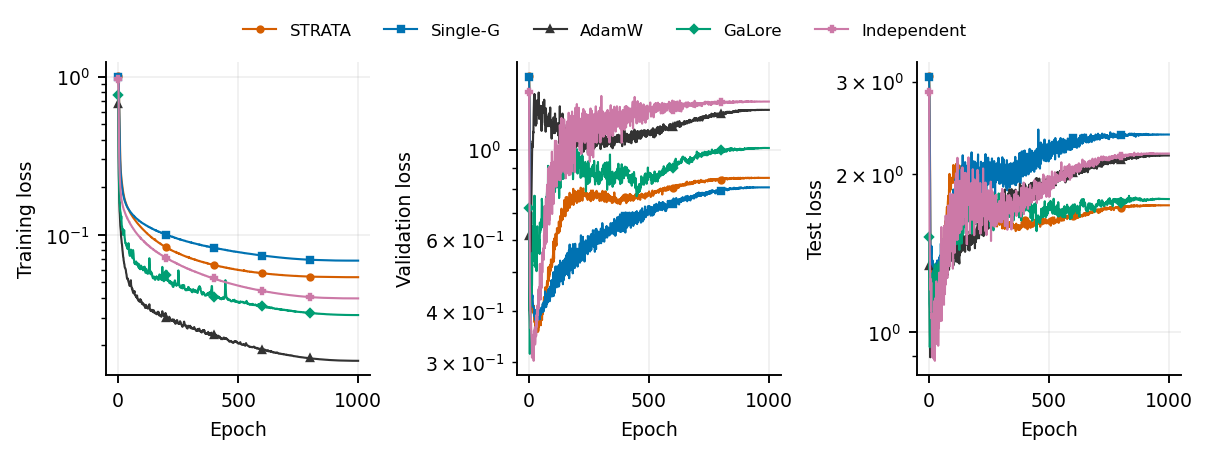
\includegraphics[width=.98\linewidth]{figures/fig_new_family_151c40f1dd.png}\caption{Complete ETTh2 / H24 loss trajectories. Left to right: training, validation, and test loss. Selection uses validation only after all candidates finish or record failure. All five methods and adverse outcomes remain visible. Curves are raw and unsmoothed.}\end{figure}
\clearpage
\paragraph{MovieLens100K / ratings complete search.} Primary metric: RMSE. Recorded candidate failures: STRATA 0, Single-G 0, AdamW 0, GaLore 0, Independent 0. Shared-CPU wall time is not isolated throughput; tensor-state size is distinct from peak memory.
\begin{table}[htbp]\centering\caption{\textbf{MovieLens100K / ratings: selected configurations and stored state.} Each method selects among six candidates on validation. Bold marks the best validation/test value; the green row identifies STRATA. Pareto status uses test quality and stored state, not peak memory.}\begin{adjustbox}{max width=\linewidth}
\begin{tabular}{lrrrrrl}\toprule Method & lr & $\xi$ & Val & Test & State MiB & Pareto\\\midrule
\rowcolor{oursbg}
STRATA & 3e-04 & 10 & 0.96257 & 0.96949 & 0.848 & \rwcross \\
Single-G & 3e-04 & 10 & 1.00521 & 1.00529 & 0.770 & \rwcross \\
AdamW & 1e-04 & -- & \textbf{0.91533} & \textbf{0.93295} & 2.584 & \rwcheck \\
GaLore & 1e-04 & -- & 0.94025 & 0.95778 & 0.692 & \rwcheck \\
Independent & 3e-04 & 10 & 1.00684 & 1.01755 & 0.833 & \rwcross \\
\bottomrule\end{tabular}
\end{adjustbox}\end{table}
\begin{figure}[!htbp]\centering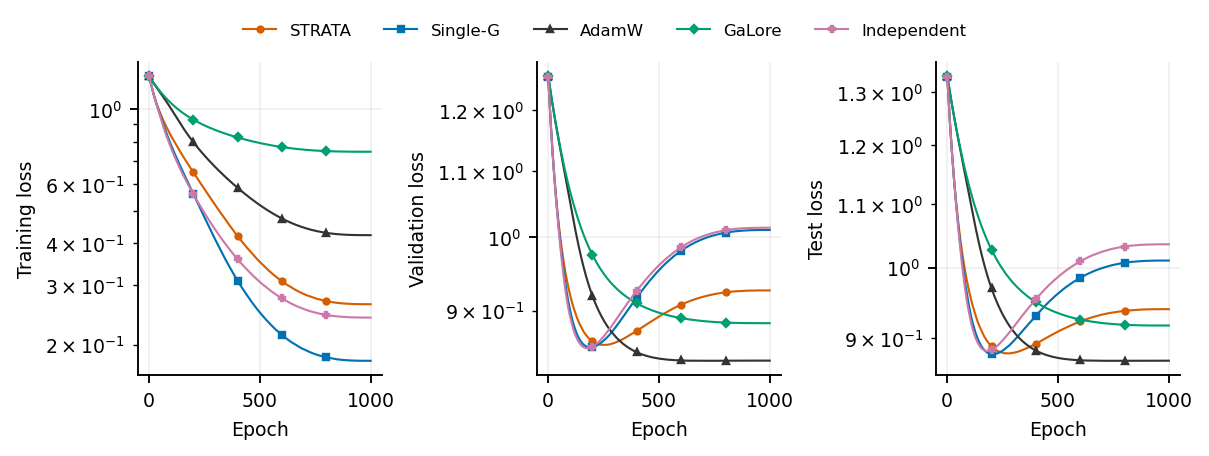
\includegraphics[width=.98\linewidth]{figures/fig_new_family_ce752a0fe4.png}\caption{Complete MovieLens100K / ratings loss trajectories. Left to right: training, validation, and test loss. Selection uses validation only after all candidates finish or record failure. All five methods and adverse outcomes remain visible. Curves are raw and unsmoothed.}\end{figure}
\clearpage
\paragraph{MovieLens1M / ratings complete search.} Primary metric: RMSE. Recorded candidate failures: STRATA 0, Single-G 0, AdamW 0, GaLore 0, Independent 0. Shared-CPU wall time is not isolated throughput; tensor-state size is distinct from peak memory.
\begin{table}[htbp]\centering\caption{\textbf{MovieLens1M / ratings: selected configurations and stored state.} Each method selects among six candidates on validation. Bold marks the best validation/test value; the green row identifies STRATA. Pareto status uses test quality and stored state, not peak memory.}\begin{adjustbox}{max width=\linewidth}
\begin{tabular}{lrrrrrl}\toprule Method & lr & $\xi$ & Val & Test & State MiB & Pareto\\\midrule
\rowcolor{oursbg}
STRATA & 3e-04 & 0.001 & 1.03092 & 1.05052 & 2.703 & \rwcross \\
Single-G & 3e-04 & 0.001 & 1.07528 & 1.09444 & 2.625 & \rwcross \\
AdamW & 1e-04 & -- & 0.96096 & 0.98066 & 9.834 & \rwcross \\
GaLore & 1e-04 & -- & \textbf{0.89748} & \textbf{0.91712} & 2.547 & \rwcheck \\
Independent & 3e-04 & 10 & 1.05453 & 1.08146 & 2.688 & \rwcross \\
\bottomrule\end{tabular}
\end{adjustbox}\end{table}
\begin{figure}[!htbp]\centering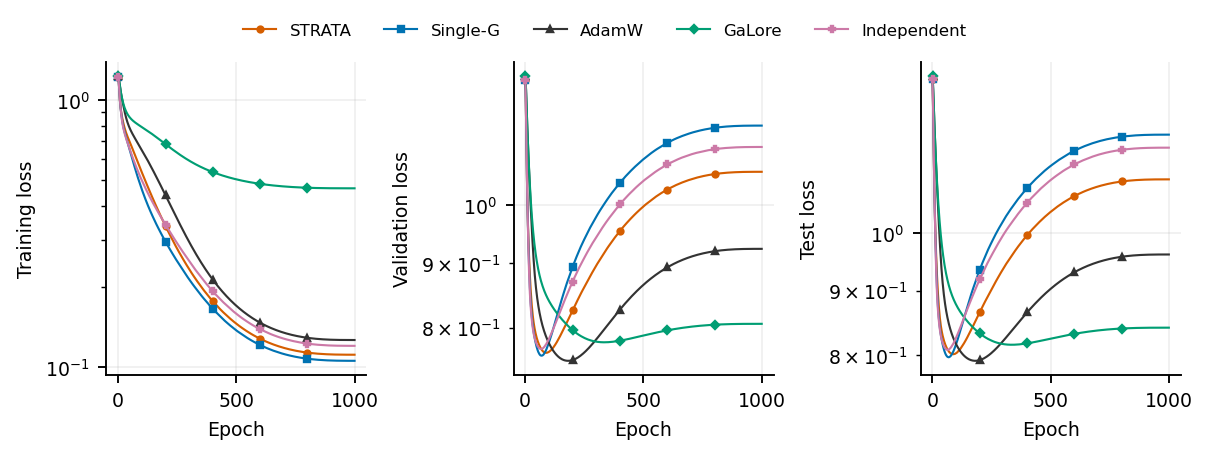
\includegraphics[width=.98\linewidth]{figures/fig_new_family_4338a23ff7.png}\caption{Complete MovieLens1M / ratings loss trajectories. Left to right: training, validation, and test loss. Selection uses validation only after all candidates finish or record failure. All five methods and adverse outcomes remain visible. Curves are raw and unsmoothed.}\end{figure}
\clearpage
\paragraph{Gas sensors / fine-tuning complete search.} Primary metric: acc. Recorded candidate failures: STRATA 0, Single-G 0, AdamW 0, GaLore 0, Independent 0. Shared-CPU wall time is not isolated throughput; tensor-state size is distinct from peak memory.
\begin{table}[htbp]\centering\caption{\textbf{Gas sensors / fine-tuning: selected configurations and stored state.} Each method selects among six candidates on validation. Bold marks the best validation/test value; the green row identifies STRATA. Pareto status uses test quality and stored state, not peak memory.}\begin{adjustbox}{max width=\linewidth}
\begin{tabular}{lrrrrrl}\toprule Method & lr & $\xi$ & Val & Test & State MiB & Pareto\\\midrule
\rowcolor{oursbg}
STRATA & 1e-03 & 0.1 & 0.86518 & 0.85453 & 0.422 & \rwcross \\
Single-G & 3e-04 & 0.001 & 0.85400 & 0.85375 & 0.305 & \rwcross \\
AdamW & 3e-03 & -- & 0.85438 & 0.82335 & 0.766 & \rwcross \\
GaLore & 1e-03 & -- & \textbf{0.90496} & \textbf{0.90656} & 0.188 & \rwcheck \\
Independent & 3e-04 & 10 & 0.82691 & 0.80659 & 0.398 & \rwcross \\
\bottomrule\end{tabular}
\end{adjustbox}\end{table}
\begin{figure}[!htbp]\centering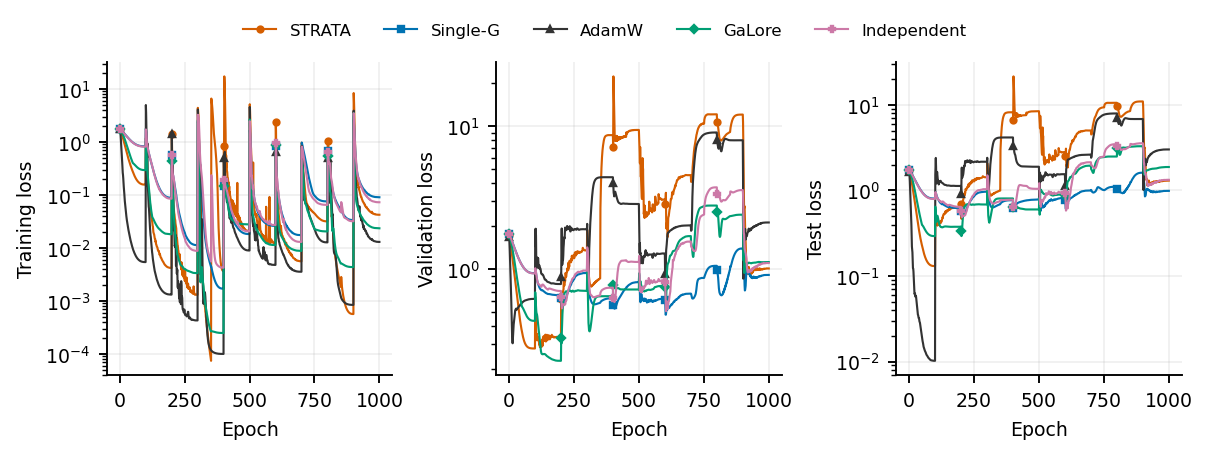
\includegraphics[width=.98\linewidth]{figures/fig_new_family_2d8b18f1f2.png}\caption{Complete Gas sensors / fine-tuning loss trajectories. Left to right: training, validation, and test loss. Selection uses validation only after all candidates finish or record failure. All five methods and adverse outcomes remain visible. Curves are raw and unsmoothed; sensor-drift evaluation averages domains seen so far and changes at domain boundaries.}\end{figure}
\clearpage
\paragraph{Gas sensors / replay complete search.} Primary metric: acc. Recorded candidate failures: STRATA 0, Single-G 0, AdamW 0, GaLore 0, Independent 0. Shared-CPU wall time is not isolated throughput; tensor-state size is distinct from peak memory.
\begin{table}[htbp]\centering\caption{\textbf{Gas sensors / replay: selected configurations and stored state.} Each method selects among six candidates on validation. Bold marks the best validation/test value; the green row identifies STRATA. Pareto status uses test quality and stored state, not peak memory.}\begin{adjustbox}{max width=\linewidth}
\begin{tabular}{lrrrrrl}\toprule Method & lr & $\xi$ & Val & Test & State MiB & Pareto\\\midrule
\rowcolor{oursbg}
STRATA & 1e-03 & 10 & \textbf{0.97487} & 0.96506 & 0.422 & \rwcheck \\
Single-G & 1e-03 & 0.001 & 0.96936 & 0.96409 & 0.305 & \rwcheck \\
AdamW & 3e-03 & -- & 0.97452 & \textbf{0.96536} & 0.766 & \rwcheck \\
GaLore & 1e-03 & -- & 0.97444 & 0.96232 & 0.188 & \rwcheck \\
Independent & 1e-03 & 10 & 0.97214 & 0.96343 & 0.398 & \rwcross \\
\bottomrule\end{tabular}
\end{adjustbox}\end{table}
\begin{figure}[!htbp]\centering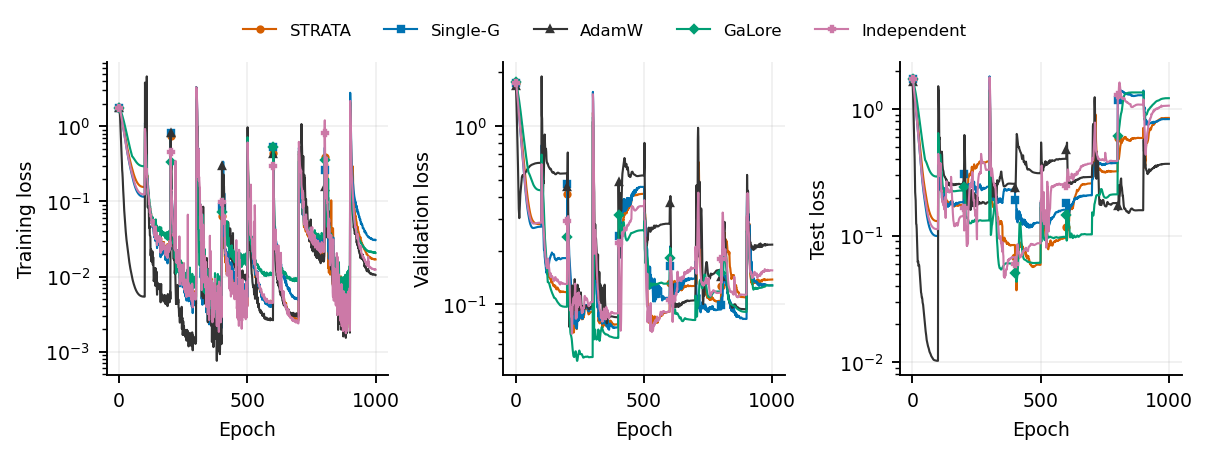
\includegraphics[width=.98\linewidth]{figures/fig_new_family_8ed4986eff.png}\caption{Complete Gas sensors / replay loss trajectories. Left to right: training, validation, and test loss. Selection uses validation only after all candidates finish or record failure. All five methods and adverse outcomes remain visible. Curves are raw and unsmoothed; sensor-drift evaluation averages domains seen so far and changes at domain boundaries.}\end{figure}
